\chapter{Discussion}
\label{ch:discussion}
This chapter discusses the results of the project and how they differ from what was expected.
We also discuss what may be done to improve the results given more time to implement changes.

\section{Expectations versus results}\label{sec:expectations-versus-results}
At the project inception, the expectations for the project were quite big.
We decided early on that we would split up the data extraction into different modules.
A CNN would be used for image classification to determine the type of receipt, with a separate module for date and price extraction whose implementation had yet to be decided.
A website would be used to allow the user to send their image to our data extraction pipeline, and also display the result for the user to confirm before sending it to a database.
The API would connect all the different modules and handle passing the information between them.
Looking back at these expectations, our end product does match these expectations, but the capabilities and results of the different modules turned out to less than what we expected.

\subsection{Supervised or unsupervised learning}\label{subsec:supervised-or-unsupervised-learning}
Early on we did not yet have access to the dataset to be used to train our models.
What we knew about the dataset was that it would be unlabeled, meaning that if we decided to use a supervised learning training method, we would have to label the data ourselves.
We also knew that Simployer preferred a solution where our model could be used on a large variety of receipts.
This made us lean towards unsupervised learning, as creating hundreds of categories for different types of receipts would be very time-consuming and likely unmanageable.
When looking into unsupervised learning for a problem such as this, we got the impression that this would be very difficult.
One person experienced in the field told us we would get a Nobel Prize if we managed to do this.
Though jokingly, this put us off the idea of unsupervised learning as the problem seemed out of scope for this project.
Now left with the method of supervised learning for our models, our expectations had to be lowered, and we decided to pivot more to a proof-of-concept product.
This meant we could limit ourselves to a lower number of categories to showcase how the project pipeline would work if given more time to implement.
Now the process of labeling data was less time-consuming as we decided to only train our models on 3 different categories of receipts.

\section{API discussion}\label{sec:api-discussion}
\subsection{.NET API}\label{subsec:.net-api2}
The decisions to utilize a .NET API was made for us by Simployer.
As explained in~\ref{sec:api-results}, our implementation of the API's

\section{Receipt category extraction with CNN}\label{sec:receipt-category-extraction-with-cnn}
After deciding to use a CNN for image classification to extract the receipt category, we expected the have a working model up and running in a short amount of time.
Early on we had a lot of issues setting up Tensorflow and CUDA on our machines, and once we got it working on one machine, the same method of installation would not work for another machine.
Once we got Tensorflow working, we also ran into issues of huge training times as Tensorflow was using the CPU to train our model, instead of the GPU.
This was fixed simply by enabling the GPU via python code, but took us quite some time and caused us to reinstall both Tensorflow and CUDA several times.

\subsection{Inconsistency between validation accuracy and pipeline testing}\label{subsec:inconsistency-between-validation-accuracy-and-pipeline-testing}
Initially we were quite happy with the results of our CNN model, with the validation accuracy after training usually being above 95\%.
After implementing the CNN module into our pipeline however, we discovered that it was not predicting the correct category nearly as often as the validation accuracy led us to believe it would.
As presented in chapter 5, when attempting to predict the receipt category via a finished model in our API, the model would often predict the wrong category despite a strong validation accuracy.
This would make more sense if we were testing the pipeline with images not contained in our dataset.
But as the validation accuracy is based on a test subset of our training dataset, we assumed testing the pipeline with images from the same dataset would have similar results.
The cause of this remains a mystery to us, but leads us to believe there is a fundamental flaw in how we are interpreting the validation metrics.

\section{Receipt date extraction with OCR}\label{sec:receipt-date-extraction-with-ocr}
Originally, the OCR module was not supposed to be used for any information extraction.
The OCR module was only designed as an image-to-text converter, as the last module in our pipeline required input-data in the form of text.
As the project approached its end-date, we had not managed to implement a working solution to extract the price and date data.
In order to finish the pipeline, so it could be demonstrated properly, a Regular Expression was added at the end of the OCR module, which simply extracts the first valid date found in the text.
This solution has some flaws, as there can be many dates found in a receipt, and no validation as to which date is likely the correct one being added.

\subsection{Issues with reliance on CNN prediction}\label{subsec:issues-with-reliance-on-cnn-prediction}
As mentioned in chapter 5 and seen in~\ref{fig:scuffedmatchresult}, the de-skew being reliant on CNN prediction has consequences for the rest of the pipeline.
This means that unless the CNN makes the correct prediction, and the de-skewing manages to properly rotate the image to a horizontal state, no text can be found in the image, as it is rendered unusable by the de-skewing.
In some cases where the CNN does correctly predict the receipt category, the de-skewing also fails, giving the same result as~\ref{fig:scuffedmatchresult}.
This is one of the biggest issues with our pipeline, as any further information extraction is no longer possible.
One way to solve this problem would be to find a way to de-skew images without relying on a template image of a given category.
This would remove the reliance on the CNN prediction.
A big benefit to this that we would be able to extract date and price information from the images even if the CNN prediction fails.
Another possible solution would be to only accept images that are taken horizontally, meaning no de-skewing would be required for the OCR to properly identify text in an image.
This solution would require the user to only submit images where the text is horizontally aligned.
In this case the CNN would probably need to be retrained as well, as much of the training data is rotated in order to account for images taken at a bad angle.

\subsection{Issues with receipt character ambiguity}\label{subsec:issues-with-receipt-character-ambiguity}
One of the issues that led to the bad date extraction of the example in chapter 5 is character ambiguity.

\begin{figure}[h]
    \center{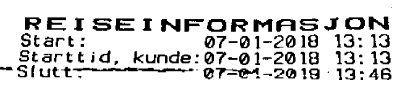
\includegraphics[width=1\textwidth]{Images/zeroletter}}
    \caption{Character ambiguity in dates}
    \label{fig:zeroletter}
\end{figure}

Figure~\ref{fig:zeroletter} shows a partition of a Norwegian receipt where all the characters representing the number
zero has a dash going through it.
This is likely being done to avoid confusion between the number zero and the character O.
However, since the receipt is in Norwegian, it creates a situation where the is confusion between the number zero and the character Ø.
This is what caused the incorrect date extraction in the example in chapter 5.
When examining the OCR text output, we could see several of the dates being listed as "Ø7-Ø1-2Ø18".
This format is not recognized by the Regular Expression for date extraction, as it is not a date format.
It is possible this issue could be solved by changing the OCR language to english, but it has not been tested, so it is unclear how it would impact the overall result of the text extraction.

\section{Price extraction with Spacy}\label{sec:price-extraction-with-spacy}
Much like the date extraction with OCR, price extraction with Spacy was added due to lack of time in order to complete our pipeline.
The results of our Spacy module was largely unusable.
Since our Spacy module uses the "MONEY" label to identify what text is currency, when none of these labels are found, only a price of -1 is given back to the API, indicating that a price has not been found.
The labels found where mostly "MISC" and "PER", the rest was empty.
This combined with very bad relation binding mostly block the possibility to have a solution that extracts the correct values.
The cause of this is because Spacy only had pre-trained models for norwegian, and not nlp pipelines.
A solution to this problem could be to train our own Spacy pipeline for norwegian.
This was however not an option duo to time constraints and lack of training data.
Another possible solution is to abandon the Spacy NER altogether, and implement an RNN as was intended initially.

\section{Overall pipeline improvements}\label{sec:overall-pipeline-improvements}